\section{Produktion}
\label{sec:ui-produktion}

\autorbeginn{Julia}

Das Produzieren der Raumschiffe wird im Bereich “Produktion” gesteuert. Das Mockup hierzu ist auf \vref{img:ui-produktion} zu sehen. 

Auch dieser Bildschirm ist in Containern aufgeteilt. Jeder Container enthält Informationen zu einem der drei Raumschifftypen, X Wing, Corellian Corvette und Millenium Falke. Ein Container enthält eine grafische Darstellung des Raumschifftyps sowie ein Hilfebutton zur näheren Erläuterung des Raumschiffes an der rechten unteren Ecke der Grafik. Betätigt man diesen Button erscheint ein PopUp-Fenster welches die weiteren Informationen enthält. Darunter befindet sich eine Tabelle welche die Anzahl der verschiedenen Bauteile enthält, die für die Produktion eines einzigen Raumschiffes von diesem Typ benötigt werden. Zudem lassen sich darunter die anfallenden Kosten pro Raumschiff ablesen. Über ein Auswahlfeld kann der Spieler die gewünschte Anzahl der zu produzierenden Raumschiffen bestimmen. Daraus errechnen sich dann die Gesamtkosten für die Produktion der Raumschiffe dieses Typs. Diese Auswahl kann der Spieler für jeden Raumschifftyp treffen.

Auf der rechten Seite des Bildschirmes kann der Spieler die Kosten aller Produktionsaufträge ablesen. Darunter befindet sich der Button “Raumschiffe produzieren” wodurch die im UseCase Diagramm auf \vref{img:fachkonzept-usecase} genannten Produktionsaufträge angelegt werden. Durch das Betätigen dieses Buttons erscheint ein PopUp-Fenster welches den Vorgang bestätigt. 

\begin{figure}[htb]
  \centering
  \fbox{
    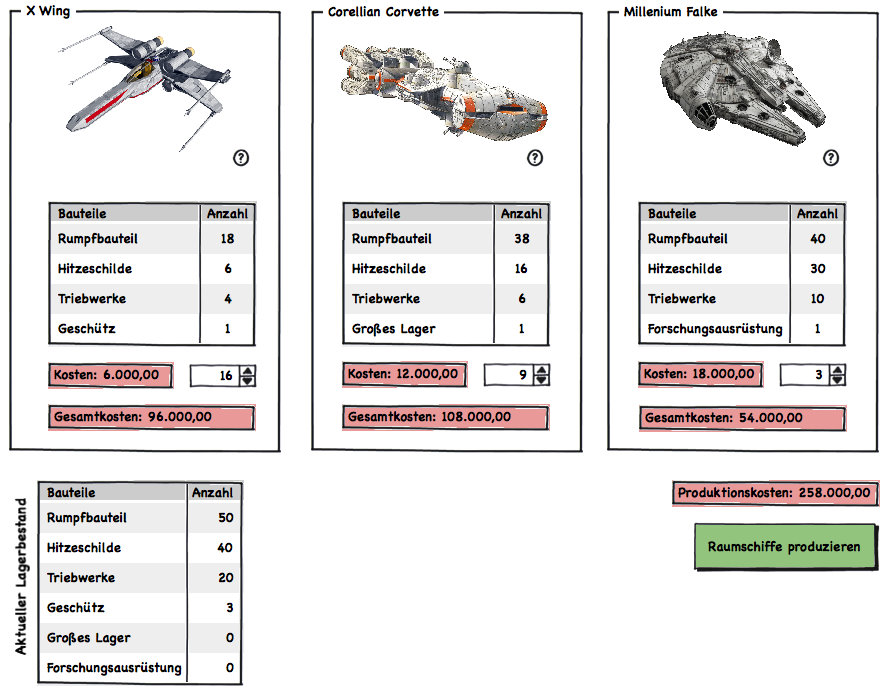
\includegraphics[width=0.9\textwidth]{40_UI/60_Produktion/Produktion.jpg}
  }
  \caption{Produktion}
  \label{img:ui-produktion}
\end{figure}

\autorende{}